\documentclass{article}
% Generated from Markdown; preserve the official workshop style.
\makeatletter
\def\input@path{{../../docs/}}
\makeatother
\PassOptionsToPackage{numbers,compress}{natbib}
\usepackage[dblblindworkshop]{neurips_2026}
\workshoptitle{Foundation Models for the Brain and Body}
\usepackage[T1]{fontenc}
\usepackage{amsmath,amssymb}
\usepackage{newunicodechar}
\newunicodechar{−}{\ensuremath{-}}
\usepackage{graphicx}
\usepackage{booktabs,longtable,array,calc}
\usepackage{microtype}
\usepackage{xcolor}
\usepackage{url}
\usepackage{hyperref}
\usepackage{placeins}
\hypersetup{hidelinks,pdfauthor={},pdftitle={}}
\setlength{\emergencystretch}{2em}
\setcounter{secnumdepth}{0}
\providecommand{\tightlist}{\setlength{\itemsep}{0pt}\setlength{\parskip}{0pt}}
\providecommand{\pandocbounded}[1]{#1}
\title{}
\author{Anonymous Author(s)}
\begin{document}
\maketitle
\section{Constructed Laterality versus Learned Movement Information: A
Source-Held-Out Controlled Evaluation of Self-Supervised Gait
Representations}\label{constructed-laterality-versus-learned-movement-information-a-source-held-out-controlled-evaluation-of-self-supervised-gait-representations}

\subsection{Abstract}\label{abstract}

We separate a geometric constraint we supply from information the
encoder actually learns during pretraining, and report what each
contributes to a movement representation. We run a source-held-out
controlled evaluation of a compact S-JEPA-inspired encoder trained on
GAVD-derived 3D pose, across five outer folds and five seeds on 625
sequences from 93 sources. Reflection augmentation reduces a strict
token-symmetry error \(q\) by 0.00843 (95\% source-bootstrap interval
{[}0.00687, 0.01020{]} on the magnitude of the reduction, roughly 7.4\%
relative to the vanilla variant), so it measurably improves consistency
under a specified anatomical mirror action. Whether that helps
prediction stays unresolved: the native learned encoder's advantage over
its matched initialization is \(-0.01798\) in source-balanced \(R^2\),
with an interval that spans zero. To isolate what pretraining
contributes, we build an odd readout whose construction guarantees
output sign reversal under reflection --- and its learned features
underperform matched initialization by 0.05874 in \(R^2\), an interval
lying entirely below zero. A separate classification pilot shows the
same ordering, with raw pose reaching 0.441 macro-F1 against 0.292 for
learned features on 20 held-out sources. Our contribution is a bounded,
artifact-verified evaluation protocol for this setting; the results
support no claim of a pretraining advantage and no claim of clinical
validity.

\section{1. Introduction}\label{introduction}

Representations of body movement are increasingly proposed as a
foundation for downstream behavioral and clinical readouts, yet a single
accuracy number rarely settles whether such a representation is doing
useful work. Two questions matter to a Brain-and-Body foundation-model
audience and answer to different evidence: whether the representation
carries information a downstream readout can use, and whether it behaves
correctly under a change of anatomical coordinate, in particular a
left/right reflection of the body. A representation can satisfy one
while failing the other, so we treat them as two separate axes of
quality.

Video-derived pose adds a nuisance that inflates apparent performance,
because a single upload often yields several excerpts of the same person
under one camera and setting, and splitting them independently lets
closely related material land on both sides of a train/test divide so a
readout scores well by recognizing the recording. We therefore evaluate
with source-held-out splits throughout encoder fitting, readout
selection, and testing, following the standard grouped-cross-validation
control against shared-upload dependence
\citep{roberts2017crossvalidation}. This is weaker than held-out-person
evaluation, because the dataset supplies no persistent identity and the
same person may recur across uploads.

Our setup is a compact skeleton joint-embedding predictive architecture
inspired by S-JEPA \citep{abdelfattah2024sjepa} and the
latent-prediction principle of I-JEPA \citep{assran2023ijepa}, trained
on pose derived from the Gait Abnormality in Video Dataset
\citep{ranjan2025gavd}. It groups 33 landmarks over time into short
patches and predicts masked latent content against an
exponential-moving-average target encoder, given no laterality label and
no diagnosis, only pose geometry. Against this backdrop the laterality
study asks whether learned features predict a signed left/right motion
contrast whose sign is defined to reverse under anatomical reflection,
whether reflection augmentation during pretraining improves how the
representation transforms under that reflection, and what an imposed
sign rule contributes once added to the readout. The signed target and
the reflection operation are constructed analytically, the readout
weights are fitted from pose-derived values, and the odd readout's sign
law --- the guarantee that a mirrored input flips the output --- is
imposed by construction, so it holds for any encoder and any fitted
weights. This keeps the learned, the fitted, and the built-in components
distinct throughout.

\textbf{Contributions.} None of the individual ingredients is new:
grouped cross-validation, linear probing, parity projection, and
building geometric structure into learning are all established
\citep{roberts2017crossvalidation, cohen2016gcnn, bronstein2021gdl}, and
our contribution is their controlled combination as a test. We give a
two-axis evaluation for movement representations, downstream predictive
information and behavior under anatomical reflection, and show that the
two can diverge, so correct sign behavior does not imply predictive
utility. We define a signed left/right motion contrast with an exact
reflection sign law and separate three claims that are easily conflated:
analytic output oddness imposed by the readout, probe-level sign
behavior, and intrinsic token equivariance of the encoder. We run this
under a leakage-controlled, source-held-out protocol with a paired
untrained-encoder floor, five outer folds, five seeds, and
source-cluster bootstrap uncertainty, which isolates what pretraining
adds beyond initialization and supplied anatomy. A classification pilot
runs as a secondary thread, comparing learned features against raw-pose
and missingness baselines. The findings are bounded: reflection
augmentation measurably improves the token-symmetry metric, its
predictive gain is unresolved against the initialization floor, and an
odd readout guarantees output sign reversal while its learned features
underperform matched initial features. We claim no pretraining
advantage, no clinical validity, and no foundation-scale result.

\section{2. Background and related
work}\label{background-and-related-work}

Our study draws on four literatures rather than extending any one of
them. Self-supervised models for articulated motion descend from
latent-prediction objectives: I-JEPA predicts the representation of
masked image regions in an embedding space rather than reconstructing
pixels \citep{assran2023ijepa}, and S-JEPA carries that idea to skeleton
sequences \citep{abdelfattah2024sjepa}, as do related schemes such as
Skeleton2vec \citep{xu2024skeleton2vec} and masked motion predictors
\citep{mao2023mamp}, while supervised graph models like ST-GCN
\citep{yan2018stgcn} remain a standard reference for skeleton action
recognition. Because latent prediction can collapse to constant
features, we regularize with the variance, invariance, and covariance
terms of VICReg \citep{bardes2022vicreg}. Our encoder is a small
independent reimplementation of the S-JEPA design trained on our own
cohort, so we neither reproduce nor rely on any published benchmark
number.

How symmetry enters a model is a second thread. Group-equivariant
networks build a transformation group into the weight-sharing structure
\citep{cohen2016gcnn}, the geometric deep learning program frames
architectures through the symmetries they respect
\citep{bronstein2021gdl}, and E(n)-equivariant graph networks give a
concrete instance for skeletal data \citep{satorras2021egnn}. When
equivariance is not wired into the layers it can be obtained at the
input or readout through data augmentation, frame averaging over the
group \citep{puny2022frame}, or a learned canonicalization map
\citep{kaba2023canonicalization}, ranging from letting the objective
discover the symmetry to guaranteeing it by construction. The two
mechanisms we study, reflection augmentation and an odd-parity readout,
are ordinary points on that spectrum; we introduce no new equivariance
algorithm and only measure where a self-supervised skeleton encoder
falls on it.

The evaluation target itself comes from the clinical-biomechanics
literature on gait symmetry, where signed left-versus-right contrasts
expressed as symmetry indices are a long-standing summary of how the two
sides of the body move
\citep{robinson1987symmetry, sadeghi2000symmetry, patterson2010symmetry, blazkiewicz2014symmetry}.
That work justifies treating a normalized left-minus-right motion
contrast as a movement quantity worth probing, though our own quantity
is a dimensionless index of estimated landmark speeds, chosen so that it
provably negates under reflection, and not validated as a clinical
asymmetry measure. Our inputs come from marker-free pose estimation,
which has made video gait analysis practical without laboratory
instrumentation \citep{hii2023markerfree}, using the 33-landmark
BlazePose schema of an on-device 3D pose estimator
\citep{grishchenko2022blazepose, mediapipePoseLandmarker}.
Self-supervised and forecasting objectives have been applied to
pose-based gait for movement-disorder severity
\citep{endo2022gaitforemer} and fine-grained abnormality detection
\citep{duan2024fsgait}; those studies ask whether a learned
representation predicts a clinical outcome, whereas we ask only whether
it carries a specific bilateral-symmetry structure that behaves
correctly when the input is mirrored.

\section{3. Methods}\label{methods}

\textbf{Cohort and unit of evaluation.} Both studies draw on the Gait
Abnormality in Video Dataset \citep{ranjan2025gavd, gavdRepo2026}, whose
distribution supplies annotations and public video links rather than raw
media, with folder labels (normal, Parkinson's, stroke, myopathic,
cerebral palsy) that this project has not validated as diagnoses. A
single upload can yield several sequences, so the \emph{source} is a
coarser unit than the \emph{sequence}, and splitting sequences
independently would let clips from one recording fall on both sides of a
train/test divide; every fold is therefore built at the source level.
The laterality study (Study B) is our primary evidence, with
pre-specified quality and target-computability gates retaining 625
sequences from 93 sources out of 642 available derived-pose archives;
the classification pilot (Study A) is a separate, earlier design on an
overlapping cohort of 639 sequences from 97 sources, so the two are
distinct designs whose counts must not be pooled. Source grouping
controls shared-upload dependence \citep{roberts2017crossvalidation},
but GAVD supplies no persistent person identifier and we do not infer
one, so source-disjoint evaluation is a more limited guarantee than
person-disjoint evaluation. Appendix A gives the per-class composition
and full attrition ledger.

\textbf{Representation learning.} Both models share a skeleton front end
that groups 33 pelvis-centered, scale-normalized BlazePose landmarks
into four-frame patches over a 64-frame window and predicts masked
latent content against an exponential-moving-average target encoder,
with neither the laterality target nor the annotation label entering the
objective. Study B uses a 96-dimensional four-layer encoder with a
two-layer Transformer predictor, trained with a centered latent
cross-entropy regularized in a two-view VICReg style
\citep{bardes2022vicreg}. The one comparison that matters here is
between a vanilla variant that never reflects a training sample and a
reflection-augmented variant that reflects each sample with probability
0.5 before its two views are generated; within a seed the two variants
share initialization, source draws, masks, views, and optimizer
schedule, so the pair stays matched. Appendix A gives the full
architecture, loss weights, and schedule.

\textbf{A signed laterality target.} The evaluation target compares
movement on the two sides of the pose. Let \(M\) negate the horizontal
coordinate and swap the full anatomical left/right landmark map,
including validity flags; applied twice it returns the input, so
\(M^2 = I\). Five landmark pairs enter the target (shoulders, knees,
ankles, heels, foot tips), with the hips excluded because
pelvis-centering makes their two velocity magnitudes algebraically
identical. For each pair \(k\) we take the median left and right speeds
\(m_{L,k}\) and \(m_{R,k}\) over paired-valid frame transitions and form
the normalized contrast and target

\[
c_k = \frac{m_{L,k} - m_{R,k}}{m_{L,k} + m_{R,k} + 10^{-8}},
\qquad
y(X) = \frac{1}{5}\sum_{k=1}^{5} c_k .
\]

Because \(M\) swaps every left landmark with its right partner,
\(y(MX) = -y(X)\) holds even for an asymmetric observed gait, which is
the property this evaluation relies on. Across the cohort the target is
small and roughly centered (mean \(-0.00607\), standard deviation
\(0.05915\)). It is a dimensionless coordinate-derived index, not a
validated clinical asymmetry measure or a marker of neural laterality
\citep{patterson2010symmetry}.

\textbf{Separating learned prediction from the imposed sign rule.} For
each of the five pairs an anatomical feature \(A(X)\) concatenates the
left-minus-right and left-plus-right token means on the shared valid
temporal support, giving 960 features supplied equally to the trained
encoder and to its recorded initialization, so any advantage of training
must appear on top of the same structure. From \(A\) we form equal-width
odd and even projections under reflection,

\[
\Phi^-(X) = \frac{A(X) - A(MX)}{\sqrt{2}},
\qquad
\Phi^+(X) = \frac{A(X) + A(MX)}{\sqrt{2}},
\]

and since \(M^2 = I\) the odd part satisfies
\(\Phi^-(MX) = -\Phi^-(X)\). The constructed odd readout is
\(h(X) = w^\top \Phi^-(X)\) with feature centering and the regression
intercept both disabled, since a nonzero intercept or feature-mean
offset would break the identity \(h(MX) = -h(X)\) that otherwise holds
for any encoder and any fitted \(w\). The weights still learn to predict
\(y\), but the sign behavior follows from the construction alone and
reveals nothing about acquired information
\citep{cohen2016gcnn, puny2022frame}. We evaluate four readout lanes ---
native, odd, odd with zero origin, and even --- each fitted for both the
learned features and their matched initialization, with the ridge
penalty selected on four inner source folds within the outer-training
set.

\textbf{Strict token-symmetry metric.} A separate test asks whether the
encoder tokens themselves transform correctly under reflection. We
compare the tokens of a mirrored input against the anatomically permuted
tokens of the original, allowing no Procrustes alignment, rotation, sign
search, or fitted transform, and report a normalized squared error \(q\)
on the jointly valid positions (Appendix A gives the exact form). A
value near zero indicates equivariance under this action, while
unrelated equal-energy representations sit near one. The metric is
uncentered, so features that are shared across inputs or insensitive to
the input can lower \(q\) without encoding anatomy, and a small value at
initialization does not by itself demonstrate learned structure; we
treat 0.10 as an operational, uncalibrated threshold.

\textbf{Estimand and uncertainty.} Study B divides the 93 eligible
sources into five stratified outer folds, each holding out 18 or 19 test
sources while the rest train the fold-local encoder and fit the readout,
so each source is a test source once and clips are weighted inversely to
their source's clip count. The primary estimand is specific: for each
seed we pool the held-out clip predictions across all five outer folds,
compute the source-balanced sequence-level \(R^2\), then average across
the five seeds. Uncertainty comes from 2,000 paired bootstrap draws that
resample the 93 source clusters, keeping each sampled source's clips and
all five seeds together. The resulting pointwise 95\% intervals are
conditional on the fitted models and the fixed split; they do not
propagate uncertainty from full retraining or from selection over splits
\citep{brodersen2010balanced, pedregosa2011scikit}.

\section{4. Results}\label{results}

We report the laterality study first because it carries the controlled
comparisons, and close with the classification pilot as supporting
context. Table 1 collects every contrast with its pointwise 95\%
source-bootstrap interval, and the figure in Appendix A shows the same
values graphically; the text below reads the table rather than repeating
it.

\textbf{Predictive value of the learned representation.} The native
learned readout on the vanilla encoder reaches an absolute \(R^2\) of
\(0.05979\), but its interval crosses zero, so on its own it does not
clear a floor of useful prediction. The paired contrast against the
encoder's own untrained initialization is more informative, because it
isolates what pretraining adds while holding fixed the variance shared
between readout and target. That difference is \(-0.01798\) with an
interval that spans zero, so the predictive gain from this pretraining
recipe is unestablished: the data neither show that pretraining helped
nor, given the interval width, establish equivalence to the untrained
representation. Reflection augmentation leaves the predictive estimates
essentially unchanged, its augmented-minus-vanilla contrast also
crossing zero.

\textbf{Reflection augmentation and token symmetry.} The strict token
metric gives a more definite reading on the geometry. Augmentation
measurably reduces the token-symmetry error relative to vanilla, by
\(-0.00843\) with an interval entirely below zero, a reduction of
roughly 7.4\%, and it is the one contrast we report whose interval lies
wholly on one side of zero. Two cautions attach to it. Both trained
variants have higher \(q\) than the initialization (\(+0.03055\) and
\(+0.02213\)), so training as configured moves the tokens away from the
approximate reflection consistency present at initialization and
augmentation only partly offsets that. And both trained variants have
absolute \(q\) intervals that cross the operational threshold of 0.10,
so neither sits wholly below it, and this one fixed swap does not
exclude other latent symmetry actions.

\textbf{An imposed sign rule does not confer predictive benefit.}
Because feature centering and the intercept are disabled and the readout
acts on the odd component \(\Phi^-\), the sign law \(h(MX) = -h(X)\)
holds for any encoder and any fitted weights, and the numerical check
confirms it: for every seed the original and mirrored predictions sum to
zero within \(10^{-6}\). That guaranteed antisymmetry does not translate
into predictive value from pretraining. The constructed odd/zero-origin
lane on the learned vanilla encoder underperforms its matched
initialization by \(-0.05874\) with an interval lying entirely below
zero, so the modest structure these lanes exploit comes from the parity
wrapper on the anatomical pairs and the learned features add nothing.

\begin{longtable}[]{@{}
  >{\raggedright\arraybackslash}p{(\linewidth - 6\tabcolsep) * \real{0.4600}}
  >{\raggedright\arraybackslash}p{(\linewidth - 6\tabcolsep) * \real{0.1200}}
  >{\raggedleft\arraybackslash}p{(\linewidth - 6\tabcolsep) * \real{0.1600}}
  >{\raggedright\arraybackslash}p{(\linewidth - 6\tabcolsep) * \real{0.2600}}@{}}
\caption{Paired laterality contrasts (Study B). \(\Delta R^2\) favors
the first-named condition when positive; \(\Delta q\) favors it when
negative. Intervals are pointwise 95\% source-bootstrap intervals
conditional on the fitted models and the fixed split.}\tabularnewline
\toprule\noalign{}
\begin{minipage}[b]{\linewidth}\raggedright
Contrast
\end{minipage} & \begin{minipage}[b]{\linewidth}\raggedright
Metric
\end{minipage} & \begin{minipage}[b]{\linewidth}\raggedleft
Estimate
\end{minipage} & \begin{minipage}[b]{\linewidth}\raggedright
95\% interval
\end{minipage} \\
\midrule\noalign{}
\endfirsthead
\toprule\noalign{}
\begin{minipage}[b]{\linewidth}\raggedright
Contrast
\end{minipage} & \begin{minipage}[b]{\linewidth}\raggedright
Metric
\end{minipage} & \begin{minipage}[b]{\linewidth}\raggedleft
Estimate
\end{minipage} & \begin{minipage}[b]{\linewidth}\raggedright
95\% interval
\end{minipage} \\
\midrule\noalign{}
\endhead
\bottomrule\noalign{}
\endlastfoot
Native learned vanilla (absolute) & \(R^2\) & \(0.05979\) &
\([-0.02527, 0.12571]\) \\
Native learned \(-\) paired init. & \(\Delta R^2\) & \(-0.01798\) &
\([-0.03851, 0.00248]\) \\
Native augmented \(-\) vanilla & \(\Delta R^2\) & \(+0.00408\) &
\([-0.00556, 0.01277]\) \\
Constructed odd/zero learned vanilla (absolute) & \(R^2\) & \(0.04302\)
& \([-0.04356, 0.11283]\) \\
Constructed odd/zero learned \(-\) matched init. & \(\Delta R^2\) &
\(-0.05874\) & \([-0.09549, -0.01740]\) \\
Initialization (absolute) & \(q\) & \(0.08322\) &
\([0.07458, 0.09404]\) \\
Vanilla (absolute) & \(q\) & \(0.11377\) & \([0.09513, 0.13843]\) \\
Augmented (absolute) & \(q\) & \(0.10534\) & \([0.08783, 0.12778]\) \\
Vanilla \(-\) initialization & \(\Delta q\) & \(+0.03055\) &
\([0.01576, 0.04763]\) \\
Augmented \(-\) initialization & \(\Delta q\) & \(+0.02213\) &
\([0.00844, 0.03934]\) \\
Augmented \(-\) vanilla & \(\Delta q\) & \(-0.00843\) &
\([-0.01020, -0.00687]\) \\
\end{longtable}

\textbf{Classification pilot (supporting context).} The earlier
five-class pilot in Study A offers context but not confirmation. On the
20 held-out sources of its one retained execution (outer fold 0, seed
42), a classifier built on raw pose features reaches a test macro-F1 of
\(0.441\), above the learned-representation lane at \(0.292\) and the
missingness-only baseline at \(0.251\), yet all three lanes miss every
stroke source in the split. Because this is a single fold and seed with
no matched untrained-encoder control and an overlapping cohort, the
controlled comparisons above neither explain nor are corroborated by it.
Appendix B gives the per-lane scores and the full configuration.

\section{5. Discussion}\label{discussion}

The main result is simple to state. In Study B we produce a physically
meaningful output whose sign flips under a left/right reflection of the
body, as a laterality index should, without that behavior depending on
the features produced during pretraining: the odd readout guarantees
\(h(MX) = -h(X)\) for any encoder and fitted weights, and reflection
augmentation measurably improves the strict token-symmetry metric, so
the correct reflection behavior comes from the group-theoretic
projection and the data augmentation we added rather than from what the
encoder learned. Against that, the pretrained representation contributes
no demonstrated predictive value over its own starting point, with the
native contrast straddling zero and the sharper odd/zero-origin lane
entirely negative; both trained variants also carry higher \(q\) than
the initialization, so on the one symmetry action we specified training
shifted the representation away from consistency even as augmentation
partly counteracted that.

Read against this workshop's themes of movement modeling and pretraining
evaluation, these findings argue that a correctly-transforming,
interpretable output is a weak signal about the content of a body
representation. A reviewer who saw only the odd readout's clean sign
reversal, or only the augmentation-driven improvement in \(q\), might
credit the encoder's features, and the matched-initialization controls
show that credit would be misplaced. Evaluating pretraining for movement
data therefore needs three things measured side by side: downstream
accuracy, a difference against a matched untrained initialization on the
same probe and split, and explicit transformation-law checks under a
specified group action. The classification pilot points to the same
caution, since there a simpler raw-pose baseline outscored the
pretrained features. Our methods --- grouped source-level splitting,
linear probing, latent masked prediction, and symmetry projection
through group-equivariant and frame-averaging machinery --- are
established rather than new, and the contribution is the controlled way
we combine them on gait data, which we offer as a robust reference point
for anyone asking whether pretraining helps a body model.

\section{6. Limitations and responsible
use}\label{limitations-and-responsible-use}

The evidence here is bounded. The two studies draw on overlapping
GAVD-derived cohorts, the same individual may recur across uploads, and
we have no reliable person-level grouping, so they are not independent
replications, must not be pooled, and can control leakage only at the
source level; with no external cohort, nothing here speaks to
generalization outside GAVD. The Study B target is a dimensionless index
engineered to satisfy \(y(MX) = -y(X)\), not a clinically validated
measure of gait asymmetry, proprioception, or neural laterality. The
strict token metric \(q\) is uncentered and probes a single
anatomical-swap action, so shared or input-insensitive features can
lower it, a low value does not by itself prove learned anatomical
structure, other symmetry actions are not excluded, and the 0.10 figure
carries no population-level meaning. The linear readouts are
small-sample, so a null probe result bounds what these probes detect,
not what the encoder contains. Study A rests on a single fold and seed
with no matched untrained-encoder control, and its checkpoint and
evaluation bundles are absent from the checkout, so its hyperparameters
follow code defaults and Study B's controls do not retroactively repair
it. None of this is foundation-scale, and we present no
neural-mechanism, multimodal-transfer, or closed-loop control evidence.

Responsible use of the underlying data carries its own constraints. GAVD
aggregates publicly posted gait videos
\citep{ranjan2025gavd, gavdRepo2026}, but public availability does not
by itself establish informed consent or permission to reuse, and gait
trajectories can be identifying even after pose extraction strips the
pixels. The project's ethics determination, data-use review, and
derived-pose release review are all unresolved, and our own reporting
sets the submission and release gate to closed; a computed readiness
index cannot override that gate. We make no clinical, surveillance, or
deployment claim, and nothing here should be read as licensing these
methods or this derived data for screening or diagnosis of any person.

\section{7. Conclusion}\label{conclusion}

Our controlled evaluation shows that a physically interpretable output
can transform correctly under body reflection by construction while the
pretrained representation shows no predictive advantage over its matched
initialization on these probes. The finding is bounded to overlapping
observational cohorts, a clinically unvalidated coordinate-derived
target, and a single specified symmetry action. Extending it would take
an independent cohort with reliable person grouping, a validated
laterality target, centered and alternative symmetry actions, and a
laterality-supervised objective matched to the same evaluation, none of
which we carry out here.

\FloatBarrier\clearpage

Appendix A. Study B implementation and reproducible detail

\begin{figure}
\centering
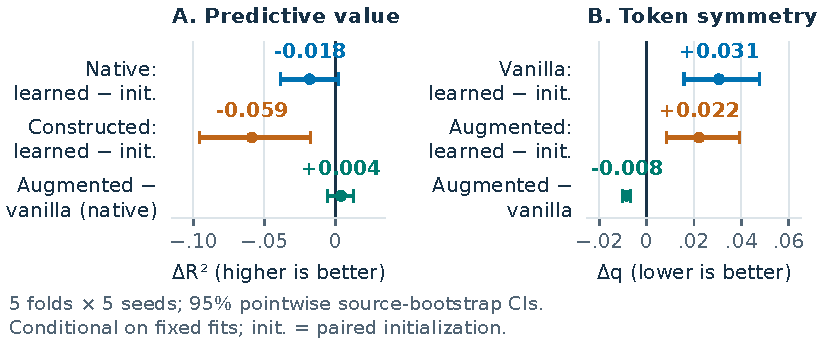
\includegraphics[width=0.72\linewidth,height=\textheight,keepaspectratio,alt={Paired laterality contrasts across five source folds and five seeds, with pointwise source-bootstrap intervals, plotting the same values as Table 1. Panel A shows predictive R\^{}2 differences (larger favors the trained representation); Panel B shows the strict token-symmetry error (smaller favors it).}]{figures/submission_laterality_effects.pdf}
\caption{Paired laterality contrasts across five source folds and five
seeds, with pointwise source-bootstrap intervals, plotting the same
values as Table 1. Panel A shows predictive \(R^2\) differences (larger
favors the trained representation); Panel B shows the strict
token-symmetry error (smaller favors it).}
\end{figure}

\textbf{Cohort composition and attrition.} The frozen GAVD inventory
describes 666 annotated sequences spanning 103 source uploads and
140,641 annotated frames. Starting from 642 available derived-pose
archives, pre-specified quality and target-computability gates retain
625 sequences from 93 sources and exclude 17. The retained cohort holds
270 normal, 39 Parkinson's, 75 stroke, 183 myopathic, and 58
cerebral-palsy sequences, drawn respectively from 29, 9, 18, 28, and 9
sources. Source roles are frozen before downstream attrition removes any
sequence.

\textbf{Skeleton front end.} Each pose sequence carries 33 BlazePose
landmarks (MediaPipe schema) with horizontal, vertical, and depth
coordinates; the pose is centered on the pelvis and scale-normalized,
and time is grouped into four-frame patches over a 64-frame window.
Twelve anatomically named landmarks are eligible masked targets: the
shoulders, hips, knees, ankles, heels, and foot tips (MediaPipe indices
11, 12, and 23 through 32). Each four-frame patch flattens its four XYZ
observations rather than averaging them, giving the encoder access to
within-patch motion, and patches with no valid content are padded out of
attention.

\textbf{Encoder, predictor, and objective.} The encoder is
96-dimensional with four layers and four attention heads, followed by a
two-layer Transformer predictor with four heads. During training up to
60\% of the eligible valid target positions are masked, limited by the
batch minimum, and the model predicts the hidden latent content against
an EMA teacher. The objective is a centered latent cross-entropy with
student and teacher temperatures 0.10 and 0.06, regularized in a
two-view VICReg style \citep{bardes2022vicreg}:

\[
L_B = L_{\mathrm{latent\,CE}} + 0.05\bigl(25\,L_{\mathrm{invariance}} + 25\,L_{\mathrm{variance}} + L_{\mathrm{covariance}}\bigr).
\]

\textbf{Optimization and augmentation.} Each of 300 epochs draws one
clip per training source and then pads to a source-uniform four batches
of 20, producing 1,200 gradient updates per encoder under AdamW at
learning rate \(10^{-3}\), betas \((0.9, 0.95)\), weight decay \(0.05\),
cosine decay, and gradient-norm clipping at 1; the EMA coefficient rises
from \(0.999\) toward 1 with target-centering coefficient \(0.9\). The
two views apply rotations up to eight degrees and XY translations up to
\(0.03\) normalized units. The vanilla variant never reflects a training
sample; the reflection-augmented variant reflects each sample with
probability \(0.5\) before the two views are generated. Within a seed
the two variants share initialization, source draws, masks, views,
optimizer schedule, and update count. Checkpoints follow a fixed
schedule with no early stopping and no validation-based selection.

\textbf{Target computation.} The five contributing pairs are shoulders,
knees, ankles, heels, and foot tips. For each pair the median left and
right speeds are taken over paired-valid transitions, meaning both
landmarks are observed at both ends of the same frame transition, with
at least eight such transitions required per pair; speeds use the
original timestamp differences and uninterpolated coordinates.

\textbf{Strict token-symmetry metric.} Let \(Z(X)\) and \(Z(MX)\) be
target-encoder tokens and \(S\) the anatomical landmark permutation on
the latent channels; on the positions \(C\) valid in both aligned views,
with no Procrustes alignment, rotation, sign search, or fitted transform
allowed, the strict error is

\[
q(X) = \frac{\lVert Z(MX) - S\,Z(X)\rVert_C^2}{\lVert Z(MX)\rVert_C^2 + \lVert S\,Z(X)\rVert_C^2}.
\]

A value near zero indicates equivariance under this action, while
unrelated equal-energy representations sit near one. The metric requires
at least eight jointly valid positions and rejects negligible-energy
representations. It is uncentered, so features shared across inputs or
insensitive to the input can lower \(q\) without encoding anatomy, and a
small value at initialization does not by itself demonstrate learned
structure; we treat 0.10 as an operational, uncalibrated threshold, and
a different joint permutation could yield a different number.

\textbf{Fitting and inner selection.} Within each outer-training set,
four inner source folds select the ridge penalty from
\(\{10^{-3}, 10^{-2}, 10^{-1}, 1, 10, 100, 1000\}\) on outer-training
embeddings only; these inner folds tune the readout and never stop
encoder training or select a checkpoint. Source-level sign accuracy and
balanced accuracy \citep{brodersen2010balanced} are reported as
secondary measures, and the fitting and scoring stack is the standard
ridge and cross-validation machinery \citep{pedregosa2011scikit}. We
report the source-balanced, seed-averaged sequence-level \(R^2\) rather
than a source-mean-target \(R^2\), which would score one aggregated
prediction per source, or a seed-ensemble score, which would average
predictions before scoring; each answers a different question.

Appendix B. Study A classification pilot

The pilot model is deliberately smaller and organized differently from
Study B. Its four-frame patches are coordinate-averaged and read by a
pooled-context MLP predictor, with the implemented loss

\[
L_A = L_{\mathrm{SmoothL1}} + 0.10\,L_{\mathrm{variance}} + 0.01\,L_{\mathrm{covariance}},
\]

where an optional condition cross-entropy term (weight \(0.10\)) is
disabled in the primary run, though the annotation labels still set a
cumulative normal-first exposure order: normal, then adding Parkinson's,
stroke, myopathic, and cerebral-palsy sequences, with earlier categories
retained. The encoder is width 64 with two layers and four heads, and
the recorded defaults are batch size 32, 20 epochs of 100 steps per
stage, learning rate \(10^{-3}\), and EMA \(0.996\). Its quality checks
retain 657 sequences from 100 sources with public metadata, 655 from 98
after media-span checks, and 639 from 97 after pose quality control.

Study A rests on a single retained execution (outer fold 0, seed 42),
and its current checkpoint and evaluation bundles are absent from the
checkout, so these hyperparameters follow code defaults, without an
independently confirmed run configuration or a matched untrained-encoder
control. On the 20 held-out sources of that fold, the three lanes score
as follows.

\begin{longtable}[]{@{}
  >{\raggedright\arraybackslash}p{(\linewidth - 6\tabcolsep) * \real{0.4200}}
  >{\raggedleft\arraybackslash}p{(\linewidth - 6\tabcolsep) * \real{0.2000}}
  >{\raggedleft\arraybackslash}p{(\linewidth - 6\tabcolsep) * \real{0.2000}}
  >{\raggedleft\arraybackslash}p{(\linewidth - 6\tabcolsep) * \real{0.1800}}@{}}
\caption{Classification pilot (Study A), 20 held-out sources of fold 0,
seed 42. Feature dimensions are at the default width. This single
execution has no matched untrained-encoder control, and all three lanes
miss every stroke source in the test split.}\tabularnewline
\toprule\noalign{}
\begin{minipage}[b]{\linewidth}\raggedright
Lane
\end{minipage} & \begin{minipage}[b]{\linewidth}\raggedleft
Feature dim
\end{minipage} & \begin{minipage}[b]{\linewidth}\raggedleft
Test macro-F1
\end{minipage} & \begin{minipage}[b]{\linewidth}\raggedleft
Balanced accuracy
\end{minipage} \\
\midrule\noalign{}
\endfirsthead
\toprule\noalign{}
\begin{minipage}[b]{\linewidth}\raggedright
Lane
\end{minipage} & \begin{minipage}[b]{\linewidth}\raggedleft
Feature dim
\end{minipage} & \begin{minipage}[b]{\linewidth}\raggedleft
Test macro-F1
\end{minipage} & \begin{minipage}[b]{\linewidth}\raggedleft
Balanced accuracy
\end{minipage} \\
\midrule\noalign{}
\endhead
\bottomrule\noalign{}
\endlastfoot
Raw pose & \(144\) & \(0.441\) & \(0.443\) \\
Learned representation & \(256\) & \(0.292\) & \(0.257\) \\
Missingness only & \(97\) & \(0.251\) & \(0.248\) \\
\end{longtable}

Appendix C. Evidence boundaries and release status

The table below records what each headline claim rests on and where its
evidentiary boundary lies. It is meant to keep the reported findings
inside the limits the data support.

\begin{longtable}[]{@{}
  >{\raggedright\arraybackslash}p{(\linewidth - 4\tabcolsep) * \real{0.2600}}
  >{\raggedright\arraybackslash}p{(\linewidth - 4\tabcolsep) * \real{0.4000}}
  >{\raggedright\arraybackslash}p{(\linewidth - 4\tabcolsep) * \real{0.3400}}@{}}
\caption{Claim, supporting evidence, and evidentiary
boundary.}\tabularnewline
\toprule\noalign{}
\begin{minipage}[b]{\linewidth}\raggedright
Claim
\end{minipage} & \begin{minipage}[b]{\linewidth}\raggedright
Evidence
\end{minipage} & \begin{minipage}[b]{\linewidth}\raggedright
Boundary
\end{minipage} \\
\midrule\noalign{}
\endfirsthead
\toprule\noalign{}
\begin{minipage}[b]{\linewidth}\raggedright
Claim
\end{minipage} & \begin{minipage}[b]{\linewidth}\raggedright
Evidence
\end{minipage} & \begin{minipage}[b]{\linewidth}\raggedright
Boundary
\end{minipage} \\
\midrule\noalign{}
\endhead
\bottomrule\noalign{}
\endlastfoot
Odd readout guarantees output sign reversal & Analytic (\(\Phi^-\) with
zero origin) plus per-seed numerical check to \(10^{-6}\) & Property of
the construction, not of learned features \\
Reflection augmentation lowers \(q\) vs.~vanilla &
\(\Delta q = -0.00843\), interval \([-0.01020, -0.00687]\) below zero &
One fixed anatomical swap; both trained variants still exceed the 0.10
threshold and the initialization \\
Pretraining predictive gain (native) & \(\Delta R^2 = -0.01798\),
interval \([-0.03851, 0.00248]\) & Interval spans zero: neither a gain
nor equivalence is established \\
Pretraining predictive gain (odd/zero) & \(\Delta R^2 = -0.05874\),
interval \([-0.09549, -0.01740]\) below zero & Trained features
underperform matched initialization on the sign-guaranteed lane \\
Classification pilot ordering & Raw pose \(0.441\) vs.~learned \(0.292\)
macro-F1 & Single fold and seed, no untrained control, overlapping
cohort \\
\end{longtable}

The project's ethics determination, data-use review, and derived-pose
release review are all unresolved. Our own reporting sets the submission
and release gate to closed, and a computed readiness index cannot
override that gate. We do not claim any approval that has not been
granted.
\clearpage
{\small
\bibliographystyle{plainnat}
\bibliography{../../docs/references}
}
\end{document}
